\documentclass{article}
\usepackage{tikz}
\usetikzlibrary{angles, quotes}
\usepackage{amssymb}
\usepackage{pgfplots}
\pgfplotsset{width=10cm,compat=1.9}
\usepgfplotslibrary{statistics}
\usepackage[left=2.54cm,right=2.54cm,top=2.54cm,bottom=2.54cm]{geometry}
\usepackage{tasks} %Paquete necesario para la producción de items horizontales para algunos ejercicios de tarea empleando el comando /begin{multicols}}{#}.../end{multicols} para ayudarnos a reducir las páginas
\usepackage{pdflscape} %comando que permite cambiar a orientación horizontal las hojas%
\usepackage{soul} %Paquete para permitir la compilación de acentos usando el comando {\hl{}}}\\
\sethlcolor{yellow(munsell)} %comando para definir el color para el subrayado usando el comando \hl
\usepackage[utf8]{inputenc}
\usepackage[spanish]{babel}
\usepackage{icomma}
\usepackage{ragged2e}
\usepackage{siunitx}
\usepackage{url}
\usepackage[colorlinks=true, urlcolor=blue,  linkcolor=black, citecolor=green]{hyperref}
\usepackage{pdfpages}
\usepackage{blindtext} %Paquete que genera texto ficticio (dummy text) con el comando: \blindtext
\usepackage{cancel} %in the preamble gives you four different modes of striking through: \cancel{text to cancel} draws a diagonal line (slash) through its argument, \bcancel{text to cancel} uses the negative slope (a backslash), \xcancel{text to cancel} draws an X (actually \cancel plus \bcancel), \cancelto{〈value〉}{〈expression〉} draws a diagonal arrow through the 〈expression〉pointing to the 〈value〉 (math-mode only)
\usepackage{csquotes}
\usepackage{afterpage}
\usepackage{parskip} 
\usepackage{float}
\usepackage{enumitem}
\usepackage{multicol}%Paquete que permite la creación aislada de columnas de texto. De esta forma se reduce la cantidad de páginas en nuestro documento
\usepackage{lipsum} %Paquete que genera texto de relleno al igual que \usepackage{blindtext}, se usa con el comando \lipsum[#-#] los #(hashtags) delimitan el número de páginas que deseamos ocupar del paquete lipsum para usarlos como relleno. 

% Definir el comando personalizado para la nota
\newcommand{\mynote}[1]{%
\begin{tikzpicture}[baseline=-0.75ex]
\node[draw, circle, fill=Apple Green!60, inner sep=2pt] (note) {\textbf{Nota:}};
\end{tikzpicture}%
\ \textit{#1}%
}

\newenvironment{Figura}
{\par\medskip\noindent\minipage{\linewidth}}
{\endminipage\par\medskip}
\usepackage{caption}
\usepackage[
backend=biber,
sorting=none,
url=true
]{biblatex} %bibliografía
\addbibresource{biblio.bib}
% Establecer el espacio entre las entradas de la bibliografía
\setlength{\bibitemsep}{1\baselineskip} % Puedes ajustar el valor según tus preferencias
\usepackage{amsmath,amsthm,amssymb,amsfonts}
\usepackage{pifont} %Permite la compilación del comando \xmark: es el símbolo de la tachita
\usepackage{mathtools} %permite la compilación de símbolos para matrices
\usepackage{empheq} %Paquete que se relaciona con \usepackage[most]{tcolorbox} para la creación de cuadros/cajas de colores para delimitar los resultados matemáticos o líneas de texto usando la línea de comando: \begin{empheq}[box={\mymath[colback=orange(webcolor)!70,drop lifted shadow]}]{equation*} \end{empheq}
\usepackage[most]{tcolorbox} %Paquete que se relaciona con \usepackage{empheq} para la creación de cuadros/cajas de colores para delimitar los resultados matemáticos o líneas de texto
\renewcommand{\qedsymbol}{$\blacksquare$}
\usetikzlibrary{positioning,decorations.pathreplacing} %Paquete que permite la compilación de llaves para cuadros sinópticos (brace diagram) 
\usepackage{schemata} %The schemata package is designed just for these brace diagrams
\usepackage{booktabs}

\newcommand\AB[2]{\schema{\schemabox{#1}}{\schemabox{#2}}} %comando o paquete necesario para crear cuadros sinópticos

\newtcbox{\mymath}[1][]{%
nobeforeafter, math upper, tcbox raise base,
enhanced, colframe=blue!30!black,
colback=blue!30, boxrule=1pt,
#1} %Comando importante para encasillar los resultados matemáticos en cajas de diferentes colores, se relaciona con los paquetes \usepackage{empheq} y \usepackage[most]{tcolorbox} 

\newenvironment{sysmatrix}[1]
{\left(\begin{array}{@{}#1@{}}}
{\end{array}\right)}
\newcommand{\ro}[1]{%
\xrightarrow{\mathmakebox[\rowidth]{#1}}%
}
\newlength{\rowidth}% row operation width
\AtBeginDocument{\setlength{\rowidth}{3em}}  %Comando importante para laproducción de lineas de operaciones entre matrices, método de Gauss o Gauss Jordan se relaciona con \newenvironment{sysmatrix}

%formato para cambiar el horario a español
\usepackage[spanish]{datetime2}
\DTMsetdatestyle{spanish}

\renewcommand{\today}{\DTMdisplaydate{\the\year}{\the\month}{\the\day }{-1}}
%%%%%%%%%%%%%%%%%%%%%%%%%%%%%%%%%%%%%%%%%

\usepackage{datetime}
\newcommand{\mycurrenttime}{\xxivtime}

%%%%%%%%%%%%%%%%%%%%%%%%%%%%%%%%%%%%%%%%%%%%%%%%%%%%%%%%%%%%%%%%%%%%%%%%%%%%%%%%%%%%%%%%%%%%%%%%%%%%%%%%%%%%%%%%%%%%%%%%%%%%%%%%%%%%%%%%%%%%%%%%%


%%%%%%%%%%%%%Caja de color para el título%%%%%%%%%%%%%%%%%%%%%%%%%%%%%%%%%%%%%%%%%%%%%%%%%%%%%%

\definecolor{myframecolor}{RGB}{1, 45, 75} % Prussian Blue
\definecolor{myboxcolor}{RGB}{0, 107, 92} % Apple Green

\newtcolorbox{mybox}{
enhanced,
colback=myboxcolor!7, % Color de fondo del cuadro
colframe=myframecolor, % Color del marco del cuadro
arc=0pt,
boxrule=1pt,
borderline west={2mm}{-10mm}{myframecolor}, % Borde en el lado izquierdo
sharp corners=southwest,
width=\linewidth,
before=\par\vspace{\bigskipamount}, % Espacio antes del cuadro
after=\par\vspace{\bigskipamount} % Espacio después del cuadro
}


\newcommand{\euler}{e} %Comando para producir letra e de euler
\newenvironment{remark}{\par\vfill\footnotesize % Vertical white space above the remark and smaller font size
\begin{list}{}{
	\leftmargin=80pt % Indentation on the left
	\rightmargin=60pt}\item\ignorespaces % Indentation on the right
\makebox[-2.5pt]{\begin{tikzpicture}[overlay]
		\node[draw=Horizon!60,line width=2.5pt,circle,fill=Horizon!25,font=\sffamily\bfseries,inner sep=4pt,outer sep=0pt] at (-19pt,5pt){\textcolor{Horizon}{Nota}};\end{tikzpicture}} % Blue Nota in a circle
\advance\baselineskip -1pt}{\end{list}\vskip5pt} % Tighter line spacing and white space after remark
\usepackage{graphicx}

\usepackage{titling}

\input{colores.tex}

%%Producir signos de cita textual``Asignatura''

\newcommand{\xmark}{\ding{55}} %%%comando que genera la tachita

\newenvironment{MyColorPar}[1]{%
\leavevmode\color{#1}\ignorespaces%
}{%
}%

%%%%%%%%%%%%%%%%%%% Título de la tarea, Nombre de alumno

\title{\textcolor{Apple Green}{\textbf{Tarea}} \textcolor{Sun}{\textbf{\#}}\textcolor{Cinnabar}{\textbf{2}} - \textbf{Ensamble microcanónico}}
\author{\emph{Julio Alfredo Ballinas García} $\boldsymbol{\mid}$ 202107583}
\date{\today}

%%%%%%%%%%%%%%%%%%% Datos de la Materia

\usepackage{fancyhdr}
\fancypagestyle{plain}{%  the preset of fancyhdr 
\fancyhf{} % clear all header and footer fields
\fancyfoot[R]{
\includegraphics[width=2cm]{LogoFCFMBUAP (1).png}}
\fancyfoot[L]{{\bfseries{\thedate{}}} a las {\bfseries{\mycurrenttime{}}} horas{} (GMT-6, H. Puebla de Zaragoza, Pue)}
\fancyhead[L]{Mecánica Estadística (NRC: 22362)}
\fancyhead[R]{\theauthor}
}
\makeatletter
\def\@maketitle{%
\newpage
\null
\vskip 1em%
\begin{center}%
\let \footnote \thanks
{\LARGE \@title \par}%
\vskip 1em%
%{\large \@date}%
\end{center}%
\par
\vskip 1em}
\makeatother

\usepackage{lipsum}  
\usepackage{cmbright}


%%%%%%%%%%%%%%%%%%%%%%%%%%%%%%%%%%%%%%%%%%%%%%%%%%%%%%%%%%%%%%%%%%%%%%%%%%%%%%%%%%%%%%%%%%%%%%%%%%%%%%%%%%%%%%%%%%%%%%%%%%%%%%%%%%%%%%%%%%%%%%%%%%%%%%%%%%%%%%%%%%%%%%%%%%%%%%%%%%%%%%%%%%%%%%%%%%%%%%

% ========= Encabezado tipo artículo + Abstract box =========
% Metadatos simples (rellénalos en el cuerpo)
\newcommand{\PaperTitle}{}        % \PaperTitle{...}
\newcommand{\PaperAuthors}{}      % \PaperAuthors{Autor1$^{a}$, Autor2$^{b}$}
\newcommand{\PaperAffils}{}       % \PaperAffils{$^{a}$ Afiliación A\\ $^{b}$ Afiliación B}
\newcommand{\PaperDates}{}        % \PaperDates{Recibido..., Revisado..., Aceptado...}
\newcommand{\PaperJournal}{}      % \PaperJournal{Food Chemistry 108 (2008) 310–315}

% Caja de encabezado (título, autores, afiliaciones, fechas)
\newtcolorbox{articleheader}{
  enhanced, colback=white, colframe=black!60,
  boxrule=0.6pt, arc=0pt,
  left=6mm, right=6mm, top=4mm, bottom=4mm,
  borderline west={2mm}{0pt}{black!70},
  before skip=6pt, after skip=10pt
}

% Caja de Abstract (con título “Abstract” al estilo revista)
\newtcolorbox{abstractbox}[1][]{
  enhanced, colback=black!3, colframe=black!60,
  boxrule=0.6pt, arc=0pt,
  left=6mm, right=6mm, top=4mm, bottom=4mm,
  title=\textbf{Abstract}, fonttitle=\bfseries,
  attach boxed title to top left={xshift=6mm, yshift*=-2mm},
  boxed title style={colback=white, colframe=black!60, boxrule=0.6pt, arc=0pt},
  before skip=6pt, after skip=6pt,
  #1
}

% Comando para “Keywords”
\newcommand{\keywords}[1]{%
  \par\smallskip\noindent\textbf{Keywords:} \textit{#1}\par
}


%%%%%%%%%%%%%%%%%%%%%%%%%%%%%%%%%%%%%%%%%%%%%%%%%%%%%%%%%%%%%%%%%%%%%%%%%%%%%%%%%%%%%%%%%%%%%%%%%%%%%%%%%%%%%%%%%%%%%%%%%%%%%%%%%%%%%%%%%%%%%%%%%%%%%%%%%%%%%%%%%%%%%%%%%%%%%%%%%%%%%%%%%%%%%%%%%%%%%%%%%%

\begin{document}



\maketitle


%%%%%%%%%%%%%%%%%%% Datos del profesor, campus y aula

\begin{mybox}
\noindent\begin{tabular}{@{}ll}
	{\bfseries{Profesor}} & Dr. Jorge Velázquez Castro\\
	\textcolor{prussianblue}{\bfseries{Campus}} / \textcolor{trueblue}{\bfseries{Facultad}}  & \textcolor{prussianblue}{\bfseries{C.U. BUAP}} /  \textcolor{trueblue}{\bfseries{FCFM}} \\
	\textcolor{prussianblue}{\bfseries{Edificio}} /  \textcolor{trueblue}{\bfseries{Salón}}    & 	\textcolor{prussianblue}{\bfseries{EMA4}} /  \textcolor{trueblue}{\bfseries{407}}   
\end{tabular} 
\end{mybox} \vspace{1cm}

\section{Instrucciones de la tarea}
\addcontentsline{toc}{section}{Instrucciones de la tarea}

\setlength{\columnsep}{2cm}
\begin{multicols}{2}

% =====================
% Problema 1
% =====================
\begin{enumerate}[label={{\textcolor{trueblue}{\textbf{Ej}. \arabic*.0}}}, start=1]
\item \textbf{Problema 1: Gas ideal 2D}

Encuentre la ecuación fundamental y las ecuaciones de estado de un gas ideal ``clásico'' confinado a 2 dimensiones.  
Hacerlo en el ensamble microcanónico.
\end{enumerate}

% =====================
% Problema 2
% =====================
\begin{enumerate}[label={{\textcolor{trueblue}{\textbf{Ej}. \arabic*.0}}}, start=2]
\item \textbf{Problema 2: Defectos de Frenkel}

Se tienen $N$ átomos iguales formando una red cristalina perfecta.  
Si se extraen $n$ átomos de sus lugares en la red (con $1 \ll n \ll N$) y se los coloca en posiciones intersticiales, se obtienen $n$ defectos de tipo Frenkel.  
El número $N'$ de posiciones intersticiales en la red es del orden de magnitud de $N$.  
Sea $W$ la energía necesaria para producir un defecto Frenkel (ver imagen).  

Halle la relación fundamental y la ecuación de estado que relaciona la energía con la temperatura.

\begin{center}
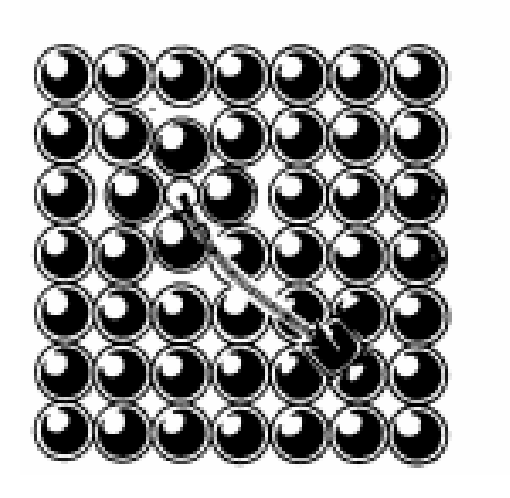
\includegraphics[width=0.65\linewidth]{p2.png}
\end{center}

\textbf{Ayuda 1}: Como $n \ll N$ asumir que $N$ es constante a pesar del número de defectos.  

\textbf{Ayuda 2}: No sólo tendrá que calcular el número de formas de acomodar los $n$ átomos en los intersticios, sino también el número de formas en que esos $n$ átomos pudieron desprenderse de la red original.
\end{enumerate}

% =====================
% Problema 3
% =====================
\begin{enumerate}[label={{\textcolor{trueblue}{\textbf{Ej}. \arabic*.0}}}, start=3]
\item \textbf{Problema 3: Cristal de Einstein en 4D}

Encuentre la ecuación fundamental y las ecuaciones de estado de un cristal de ``Einstein'' (cuántico) en 4 dimensiones.  
Realizar los cálculos en el ensamble microcanónico.
\end{enumerate}

% =====================
% Problema 4
% =====================
\begin{enumerate}[label={{\textcolor{trueblue}{\textbf{Ej}. \arabic*.0}}}, start=4]
\item \textbf{Problema 4: Tres niveles energéticos}

Considere un sistema de $N$ partículas, las cuales pueden acceder a tres niveles energéticos.  
La hamiltoniana del sistema es

\[
\mathcal{H} = h \sum_{i=1}^{N} \sigma_i^2,
\]

donde $\sigma_i = 1, 0, -1$, $h$ es una constante positiva.  

Use el ensamble microcanónico para determinar la entropía para este sistema y las ecuaciones de estado.  

Recuerde que
\[
(1+x)^n = \sum_{k=0}^n \frac{n!}{(n-k)! \, k!} x^k.
\]
\end{enumerate}

\end{multicols}


\tableofcontents \vspace{2cm}

% =====================
% Problema 1
% =====================
\begin{enumerate}[label={{\textcolor{trueblue}{\textbf{Ej}. \arabic*.0}}}, start=1]
\item \textbf{Problema 1: Gas ideal 2D}

Encuentre la ecuación fundamental y las ecuaciones de estado de un gas ideal ``clásico'' confinado a 2 dimensiones.  
Hacerlo en el ensamble microcanónico.
\end{enumerate}
\section*{Problema 1}
\addcontentsline{toc}{section}{Problema 1}

\textcolor{Cinnabar}{\textbf{Solución}}:

\paragraph{Ecuación fundamental y representaciones.}
En la \textbf{representación energética} \(\varepsilon=\varepsilon(S,V,N)\),
\[
\mathrm d\varepsilon
= \underbrace{\left(\frac{\partial \varepsilon}{\partial S}\right)_{V,N}}_{T}\mathrm dS
+ \underbrace{\left(\frac{\partial \varepsilon}{\partial V}\right)_{S,N}}_{-P}\mathrm dV
+ \underbrace{\left(\frac{\partial \varepsilon}{\partial N}\right)_{S,V}}_{\mu}\mathrm dN.
\]
En la \textbf{representación entrópica} \(S=S(\varepsilon,V,N)\), las ecuaciones de estado son
\[
\frac{1}{T}=\left(\frac{\partial S}{\partial \varepsilon}\right)_{V,N},\qquad
\frac{P}{T}=\left(\frac{\partial S}{\partial V}\right)_{\varepsilon,N},\qquad
-\frac{\mu}{T}=\left(\frac{\partial S}{\partial N}\right)_{\varepsilon,V}.
\]
En 2D sustituiremos \(V\to A\) (área) y entenderemos \(P\) como \emph{presión superficial} (conjugada a \(A\)).

\paragraph{Postulado microcanónico.}
Definimos el \emph{volumen en fase} bajo la hipersuperficie de energía \(\varepsilon\):
\begin{align}
\omega(\varepsilon)&=\frac{1}{N!\,h^{2N}}\!\!\int_{H(\mathbf r,\mathbf p)\le \varepsilon}\!\!\mathrm d^{2N}r\,\mathrm d^{2N}p,
&
\Omega(\varepsilon)&\equiv \frac{\partial \omega}{\partial \varepsilon}. \nonumber
\end{align}

\noindent
donde:
\begin{itemize}
  \item \(\mathbf{r}=(\mathbf{r}_1,\ldots,\mathbf{r}_N)\) representa las \textbf{coordenadas espaciales} de las \(N\) partículas, cada una en el plano bidimensional \(\mathbb{R}^2\).  
 Es la colección de todas las “posiciones posibles” de las partículas dentro de la caja.  
  Si conoces todas las \(\mathbf{r}_i\), sabes exactamente dónde está cada partícula del gas.

  \item \(\mathbf{p}=(\mathbf{p}_1,\ldots,\mathbf{p}_N)\) son los \textbf{momentos lineales} asociados a cada partícula.  
  Cada \(\mathbf{p}_i\) nos dice “qué tan rápido y hacia dónde” se mueve la partícula \(i\).  
  En el espacio de fases, los pares \((\mathbf{r}_i,\mathbf{p}_i)\) definen completamente el microestado de cada partícula.

  \item \(H(\mathbf r,\mathbf p)\) es el \textbf{Hamiltoniano}, la función que mide la \emph{energía total} del sistema.  
  Para un gas ideal clásico sin potencial, solo depende de los momentos:
  \[
  H(\mathbf r,\mathbf p)=\sum_{i=1}^{N}\frac{\mathbf p_i^{2}}{2m}.
  \]
  Recordemos que cada momento lineal se define como \(\mathbf{p}_i = m\,\dot{\mathbf{r}}_i\),  
  de modo que la energía cinética de cada partícula es \(\tfrac{1}{2}m\dot{\mathbf{r}}_i^{\,2} = \mathbf{p}_i^{2}/(2m)\).  
  Así, toda la energía del gas proviene del movimiento de sus partículas.  
  Si ninguna partícula se mueve, \(H=0\); si todas se mueven más rápido, \(H\) crece proporcionalmente al cuadrado de sus velocidades.

  \item \(\mathrm d^{2N}r\,\mathrm d^{2N}p\) es el \textbf{elemento de volumen del espacio de fases}.  
  Es como un tablero gigante donde cada eje representa una coordenada o un momento de alguna partícula; entonces, cada punto de ese tablero describe un posible \emph{microestado} del sistema.  
  El diferencial \(\mathrm d^{2N}r\,\mathrm d^{2N}p\) mide un pequeño volumen dentro de ese universo de configuraciones posibles.

  \item \(h\) es la \textbf{constante de Planck}.  
  Se introduce para que el volumen total del espacio de fases sea \emph{adimensional} (sin unidades físicas), ya que en mecánica cuántica el tamaño mínimo distinguible de una celda en el espacio de fases es del orden de \(h^{2N}\).  
  En otras palabras, \(h\) actúa como una “regla de conteo”: delimita qué tan finamente podemos subdividir el espacio de fases.

  \item \(N!\) corrige la \textbf{indistinguibilidad} de las partículas idénticas.  
  Si intercambiamos dos partículas iguales, el sistema no cambia físicamente, aunque sus etiquetas sí.  
  Para evitar contar dos veces el mismo microestado, dividimos entre \(N!\).

  \item \(\omega(\varepsilon)\) representa el \textbf{volumen total del espacio de fases} accesible al sistema con energía menor o igual a \(\varepsilon\).  
  Es, esencialmente, la cantidad de microestados compatibles con un límite energético máximo.  
  En el lenguaje de Feynman: “contamos todas las formas posibles en que las partículas pueden moverse sin pasarse de cierto nivel de energía”.

  \item \(\Omega(\varepsilon)=\dfrac{\partial \omega}{\partial \varepsilon}\) es la \textbf{densidad de estados}, que mide cuántos microestados existen exactamente para una energía dada.  
  Si \(\omega\) mide el volumen acumulado, \(\Omega\) sería su “pendiente”: el número de configuraciones justo en el borde de la energía \(\varepsilon\).  
  Físicamente, describe cuán densamente se agrupan los microestados en torno a una energía específica.
\end{itemize}


\noindent
Usaremos \(\omega(\varepsilon)\) como función base de conteo de microestados.

\paragraph{Gas ideal clásico 2D.}

El sistema es un gas ideal \textbf{clásico} confinado en dos dimensiones, donde el Hamiltoniano es puramente cinético:
\[
H(\mathbf r,\mathbf p)=\sum_{i=1}^{N}\frac{\mathbf p_i^{\,2}}{2m},
\qquad \mathbf p_i\in\mathbb R^2.
\]

\medskip
Dado que \(H\) no depende de las posiciones, la integral en el espacio de fases puede separarse en dos partes independientes: una puramente \emph{espacial} (asociada a las posiciones) y otra \emph{en momentos} (asociada a las velocidades de las partículas). Así, el volumen total en el espacio de fases es simplemente el producto de ambas contribuciones:
\begin{equation*}
\begin{split}
\omega(\varepsilon)
&=\frac{1}{N!\,h^{2N}}
\int \mathrm d^{2N}r
\int_{\sum_{i}\frac{\mathbf p_i^{2}}{2m}\le \varepsilon}\mathrm d^{2N}p.
\end{split}
\end{equation*}

\noindent
\textbf{Interpretación física:}  
Cada punto del espacio de fases \((\mathbf{r},\mathbf{p})\) representa un posible \emph{microestado} del gas, es decir, una configuración completa donde conocemos tanto la posición como el momento de cada partícula.  
Como el Hamiltoniano no depende de \(\mathbf{r}\), el gas puede ocupar cualquier posición en el área \(A\) con la misma probabilidad. Por ello, la integral sobre las posiciones se simplifica drásticamente:

\[
\int \mathrm d^{2N}r
=\int_A \mathrm d^2r_1\cdots\int_A \mathrm d^2r_N
= A^N.
\]

\noindent
Esto significa que hay \(A^N\) formas equivalentes de ubicar las partículas en el plano: cada partícula puede estar en cualquier punto del área disponible.  
Toda la física, entonces, queda contenida en la parte en momentos, que depende de la energía total accesible.

\vspace{1em}
\textbf{Integración sobre los momentos:}
La restricción \(\sum_{i=1}^{N}\mathbf p_i^{2}/(2m)\le \varepsilon\) define una \emph{hiperesfera} (bola \(2N\)-dimensional) de radio \(R=\sqrt{2m\varepsilon}\) en el espacio de momentos. Contar microestados cinéticos equivale a medir el \emph{volumen} de esa bola.

\medskip
Partimos de la integral en el espacio de momentos (aún en coordenadas cartesianas):
\begin{equation*}
\begin{split}
\underbrace{\int_{\sum_{i}\frac{\mathbf p_i^{2}}{2m}\le \varepsilon}\!\!\mathrm d^{2N}p}_{\text{volumen en momentos}}
&=\int_{\sum_{\alpha=1}^{2N}p_\alpha^{2}\le 2m\varepsilon}\!\!\mathrm d p_1\cdots \mathrm d p_{2N}.
\end{split}
\end{equation*}

Cambiamos a \emph{coordenadas esféricas} en \(\mathbb R^{2N}\). El Jacobiano aporta el factor \(\rho^{2N-1}\) y aparece el área de la esfera unidad \(S_{2N-1}\):
\begin{equation*}
\begin{split}
\mathrm d^{2N}p
=\underbrace{\rho^{2N-1}\,\mathrm d\rho}_{\text{Jacobiano radial}}
\;\underbrace{\mathrm d\Omega_{2N-1}}_{\text{ángulos}},
\qquad
\int \mathrm d\Omega_{2N-1}=S_{2N-1}
=\frac{2\,\pi^{N}}{\Gamma(N)}.
\end{split}
\end{equation*}

Así, la integral cartesiana se vuelve una integral radial desde \(0\) hasta \(R=\sqrt{2m\varepsilon}\):
\begin{equation*}
\begin{split}
\int_{\sum_{i}\frac{\mathbf p_i^{2}}{2m}\le \varepsilon}\!\!\mathrm d^{2N}p
&=\int_{0}^{R}\!\!\left(\int \mathrm d\Omega_{2N-1}\right)\rho^{2N-1}\,\mathrm d\rho
=\int_{0}^{R}\! S_{2N-1}\,\rho^{2N-1}\,\mathrm d\rho.
\end{split}
\end{equation*}

Integramos en \(\rho\) (observa la \(\underbrace{~}_{\text{primitiva}}\)):
\begin{equation*}
\begin{split}
\int_{0}^{R} \rho^{2N-1}\,\mathrm d\rho
=\underbrace{\frac{R^{2N}}{2N}}_{\text{primitiva en }[0,R]},
\qquad\Rightarrow\qquad
\int_{0}^{R} S_{2N-1}\,\rho^{2N-1}\,\mathrm d\rho
= S_{2N-1}\,\frac{R^{2N}}{2N}.
\end{split}
\end{equation*}

Sustituyendo \(S_{2N-1}=\dfrac{2\,\pi^{N}}{\Gamma(N)}\) y \(R^{2N}=(2m\varepsilon)^{N}\):
\begin{equation*}
\begin{split}
\int_{\sum_{i}\frac{\mathbf p_i^{2}}{2m}\le \varepsilon}\!\!\mathrm d^{2N}p
&=\frac{2\,\pi^{N}}{\Gamma(N)}\cdot \frac{(2m\varepsilon)^{N}}{2N}
=\frac{\pi^{N}}{\Gamma(N+1)}(2m\varepsilon)^{N}
=\frac{\pi^{N}}{N!}\,(2m\varepsilon)^{N}.
\end{split}
\end{equation*}

\medskip
\textbf{Espacio de posiciones y conteo total.}
Como \(H\) no depende de las posiciones, cada \(\mathrm d^{2}r_i\) integra sobre el área total \(A\), y las \(N\) partículas contribuyen de forma independiente:
\begin{equation*}
\begin{split}
\underbrace{\int \mathrm d^{2N}r}_{\text{todas las posiciones}}
=\prod_{i=1}^{N}\left(\int_{A}\mathrm d^{2}r_i\right)
=\underbrace{A\times \cdots \times A}_{N\ \text{factores}}
=A^{N}.
\end{split}
\end{equation*}

Por tanto, el volumen de fase accesible (con las normalizaciones estándar \(1/(N!\,h^{2N})\)) es
\begin{equation*}
\begin{split}
\omega(\varepsilon)
=\frac{1}{N!\,h^{2N}}
\underbrace{\left(\int \mathrm d^{2N}r\right)}_{\displaystyle A^{N}}
\underbrace{\left(\int_{\sum_{i}\frac{\mathbf p_i^{2}}{2m}\le \varepsilon}\!\!\mathrm d^{2N}p\right)}_{\displaystyle \frac{\pi^{N}}{N!}(2m\varepsilon)^{N}}
=\frac{A^{N}}{h^{2N}}\,
\frac{\pi^{N}(2m\varepsilon)^{N}}{(N!)^{2}}.
\end{split}
\end{equation*}

\medskip
\textbf{Entropía y ecuación fundamental.}
\begin{equation*}
\begin{split}
S(\varepsilon,A,N)
&=k_B\ln \omega(\varepsilon)
= k_B\Big[
N\ln A+N\ln(2\pi m\varepsilon)-2N\ln h-2\ln(N!)
\Big].
\end{split}
\end{equation*}
Usando Stirling \(\ln N!\simeq N\ln N-N\) (para \(N\gg 1\)):
\begin{equation*}
\begin{split}
S(\varepsilon,A,N)
= N k_B\!\left[
\ln\!\left(\frac{A}{N}\right)
+\ln\!\left(\frac{2\pi m}{h^{2}}\right)
+\ln\!\left(\frac{\varepsilon}{N}\right)
+2
\right].
\end{split}
\end{equation*}

\medskip
\textbf{Ecuaciones de estado (2D).}
\begin{equation*}
\begin{split}
\frac{1}{T}
=\left(\frac{\partial S}{\partial \varepsilon}\right)_{A,N}
\ \Rightarrow\ 
\varepsilon= N k_B T,
\qquad
\frac{P}{T}
=\left(\frac{\partial S}{\partial A}\right)_{\varepsilon,N}
\ \Rightarrow\ 
P\,A= N k_B T.
\end{split}
\end{equation*}
Para el potencial químico:
\begin{equation*}
\begin{split}
-\frac{\mu}{T}
=\left(\frac{\partial S}{\partial N}\right)_{\varepsilon,A}
= k_B\ln\!\left[\frac{A}{N}\frac{2\pi m}{h^{2}}\frac{\varepsilon}{N}\right]
\ \Rightarrow\
\mu=-k_B T\ln\!\left(\frac{A}{N\,\lambda_T^{2}}\right),
\quad
\lambda_T=\frac{h}{\sqrt{2\pi m k_B T}}.
\end{split}
\end{equation*}

\begin{empheq}[box={\mymath[colback=Apple Green!20,drop lifted shadow]}]{align*}
\text{Ecuación fundamental (2D):}\quad
S(\varepsilon,A,N)=
N k_B\!\left[
\ln\!\left(\frac{A}{N}\right)
+\ln\!\left(\frac{2\pi m}{h^{2}}\right)
+\ln\!\left(\frac{\varepsilon}{N}\right)
+2
\right] \\[6pt]
\text{Relación energía–temperatura:}\quad
\varepsilon = N k_B T \\[6pt]
\text{Ecuación de estado (2D):}\quad
P\,A = N k_B T \\[6pt]
\text{Potencial químico:}\quad
\mu = -\,k_B T\,\ln\!\left(\frac{A}{N\,\lambda_T^{2}}\right),
\qquad
\lambda_T=\frac{h}{\sqrt{2\pi m k_B T}}
\end{empheq}

\medskip
\textbf{Régimen clásico:}\quad
\(\displaystyle \frac{A}{N}\gg \lambda_T^{2}\), con \(\displaystyle \lambda_T=\frac{h}{\sqrt{2\pi m k_B T}}\). \vspace{0.5cm}

% =====================
% Problema 2: Defectos de Frenkel
% =====================
\begin{enumerate}[label={{\textcolor{trueblue}{\textbf{Ej}. \arabic*.0}}}, start=2]
\item \textbf{Problema 2: Defectos de Frenkel}

\textcolor{Cinnabar}{\textbf{Solución: descripción física y estadística}}

\vspace{0.6em}
Imaginemos un cristal iónico perfectamente ordenado, donde cada átomo o ion ocupa un sitio bien definido de la red.  
Sin embargo, a temperatura finita, no todo permanece perfecto: algunos átomos adquieren suficiente energía térmica para abandonar su sitio regular y desplazarse hacia una posición intersticial (un pequeño hueco dentro de la red).  
Al hacerlo, dejan tras de sí una \emph{vacante} y crean al mismo tiempo una \emph{ocupación intersticial}.  
Este par (vacante + intersticial) constituye lo que se conoce como un \textbf{defecto de Frenkel}.

Cada defecto requiere una energía \(W\) para formarse, de modo que si el cristal tiene \(n\) de estos defectos, su energía interna total asociada a la formación de defectos es:
\[
U(n) = n\,W.
\]
De aquí se deduce que el número de defectos está directamente ligado a la energía mediante:
\[
n = \frac{U}{W}, \qquad 1 \ll n \ll N,
\]
donde \(N\) es el número de sitios regulares (átomos en la red) y \(N'\) el número de posiciones intersticiales disponibles.  
En general, \(N\) y \(N'\) son del mismo orden de magnitud (\(N' \sim N\)).

\vspace{1em}
\textbf{1. Construcción del espacio de microestados.}  
En la descripción microcanónica, lo fundamental es contar \emph{cuántos microestados} son posibles para un valor dado de energía \(U\), es decir, de \(n\).  
A ese número lo llamamos \(\Omega\), el \emph{número de microestados compatibles con la energía}.  
Este número encierra toda la información estadística del sistema:
\[
\Omega(N, N'; n) \;=\; \text{número de configuraciones posibles con } n \text{ defectos}.
\]

Cada microestado se obtiene al decidir:
\begin{itemize}
  \item qué \(n\) sitios de la red \emph{quedan vacantes}, y
  \item qué \(n\) intersticios \emph{son ocupados}.
\end{itemize}
Estas dos elecciones son independientes, de modo que el número total de combinaciones posibles es el producto:
\[
\underbrace{\Omega(N,N';n)}_{\text{número total de microestados}} \;=\;
\underbrace{\binom{N}{n}}_{\text{vacantes en la red}} \times
\underbrace{\binom{N'}{n}}_{\text{ocupaciones intersticiales}}.
\]

\textit{Comentario físico:} cada combinación distinta de vacantes e intersticios representa una microconfiguración posible del cristal.  
No importa qué átomo individual se mueve, pues los átomos son indistinguibles: sólo importa qué posiciones quedan vacías y cuáles ocupadas.  
Aquí se usa la \textbf{Ayuda 2}: contar tanto el “origen” (vacantes) como el “destino” (intersticios).

\vspace{1em}
\textbf{2. Postulado microcanónico.}  
El ensamble microcanónico asume que todos los microestados accesibles a energía \(U\) son igualmente probables.  
Por tanto, la entropía \(S\) del sistema está dada por el postulado fundamental de Boltzmann:
\[
S(U,N,N') = k_B \ln \Omega(N,N'; n),
\qquad n=\frac{U}{W}.
\]
Sustituyendo la expresión de \(\Omega\):
\[
S(U,N,N') = k_B\!\left[\ln \binom{N}{U/W} + \ln \binom{N'}{U/W}\right].
\]

\vspace{1em}
\textbf{3. Aproximación de Stirling y relación fundamental.}  
Cuando \(N, N', n\gg 1\), aplicamos la aproximación de Stirling:
\(\ln m! \simeq m\ln m - m\).  
Entonces:
\[
\begin{split}
S(U,N,N') \simeq k_B\Big\{&
\underbrace{N\ln N - n\ln n - (N-n)\ln(N-n)}_{\text{vacantes en la red}} \\
&+\underbrace{N'\ln N' - n\ln n - (N'-n)\ln(N'-n)}_{\text{ocupaciones intersticiales}}
\Big\}.
\end{split}
\]
Esta expresión constituye la \emph{relación fundamental del sistema} \(S=S(U;N,N')\).

\vspace{1em}
\textbf{4. Ecuación de estado.}  
A partir de la definición termodinámica,
\[
\frac{1}{T} = \left(\frac{\partial S}{\partial U}\right)_{N,N'},
\]
y usando \(U = nW\), tenemos:
\[
\frac{1}{T} = \frac{1}{W}\left(\frac{\partial S}{\partial n}\right)_{N,N'}.
\]
Calculamos la derivada con respecto a \(n\):
\[
\frac{\partial S}{\partial n} = k_B\!\left[
\ln\!\left(\frac{N-n}{n}\right) + \ln\!\left(\frac{N'-n}{n}\right)
\right]
= k_B\ln\!\left(\frac{(N-n)(N'-n)}{n^2}\right).
\]
Así, obtenemos:
\[
\frac{1}{T} = \frac{k_B}{W}\ln\!\left(\frac{(N-n)(N'-n)}{n^2}\right),
\]
o equivalentemente:
\[
\exp\!\left(\frac{W}{k_B T}\right)
= \frac{(N-n)(N'-n)}{n^2}.
\]
Esta es la \textbf{ecuación de estado} del sistema, que relaciona el número de defectos \(n\) con la temperatura \(T\).

\vspace{1em}
\textbf{5. Solución explícita y límites.}  
Definimos \(x = \exp(W/k_B T)\).  
Despejamos \(n\) resolviendo:
\[
x n^2 = (N-n)(N'-n) = NN' - (N+N')n + n^2.
\]
Reordenando:
\[
(x-1)n^2 + (N+N')n - NN' = 0,
\]
cuya solución positiva es:
\[
n(T)=\frac{-(N+N')+\sqrt{(N+N')^2+4(x-1)NN'}}{2(x-1)}, \qquad x=e^{W/k_BT}.
\]
Como \(U = Wn(T)\), tenemos también la dependencia energética \(U(T)\).

\vspace{1em}
\textbf{6. Límite de bajas concentraciones (diluido).}  
Cuando \(n\ll N, N'\), los defectos son escasos y podemos aproximar:
\[
N-n\simeq N, \qquad N'-n\simeq N'.
\]
En tal caso:
\[
e^{W/k_BT}\simeq \frac{NN'}{n^2},
\quad \Rightarrow \quad
n(T)\simeq \sqrt{NN'}\,e^{-W/(2k_BT)},
\]
\[
U(T)\simeq W\sqrt{NN'}\,e^{-W/(2k_BT)}.
\]

\vspace{1em}
\textbf{Interpretación física:}  
La ley exponencial \(e^{-W/(2k_BT)}\) muestra que la probabilidad de formar defectos decrece rápidamente con la energía de formación \(W\) y aumenta con la temperatura.  
Así, a bajas \(T\), el cristal es casi perfecto; pero conforme la temperatura crece, los defectos aparecen de forma natural por agitación térmica.

% ===== Bloque de resultados en empheq =====
\begin{empheq}[box={\mymath[colback=Apple Green!20,drop lifted shadow]}]{align*}
\text{Relación fundamental (microcanónica):}\quad
& S(U,N,N') = k_B\ln\binom{N}{U/W} + k_B\ln\binom{N'}{U/W}.
\\[6pt]
\text{Ecuación de estado exacta:}\quad
& e^{W/k_BT} = \dfrac{(N-\tfrac{U}{W})(N'-\tfrac{U}{W})}{(\tfrac{U}{W})^2}.
\\[6pt]
\text{Solución general:}\quad
& n(T) = \dfrac{-(N+N')+\sqrt{(N+N')^2+4(e^{W/k_BT}-1)NN'}}{2(e^{W/k_BT}-1)}, 
\qquad U(T)=Wn(T).
\\[6pt]
\text{Límite diluido:}\quad
& n(T)\simeq \sqrt{NN'}\,e^{-W/(2k_BT)}, 
\qquad U(T)\simeq W\sqrt{NN'}\,e^{-W/(2k_BT)}.
\end{empheq}
% ==========================================

\vspace{0.6em}
\textbf{7. Dónde se aplicaron las ayudas.}
\begin{itemize}
  \item \textbf{Ayuda 1:} \(n\ll N\Rightarrow N\) constante.  
  Se aplica al suponer que la creación de pocos defectos no altera significativamente el número total de sitios.  
  Aparece al fijar \(N=\text{cte.}\) en la primera ecuación y en el límite diluido \(N-n\simeq N\).
  \item \textbf{Ayuda 2:} conteo doble (origen y destino).  
  Se aplica al construir \(\Omega=\binom{N}{n}\binom{N'}{n}\), donde se cuentan simultáneamente las posibles vacantes y los intersticios ocupados.
\end{itemize}

\vspace{0.7em}
La estructura combinatoria y el uso de \(\Omega\) garantizan que la entropía sea una medida del \emph{desorden configuracional}.  
El logaritmo convierte el número de microestados en una magnitud extensiva.  
Así, la teoría estadística predice no sólo la probabilidad de formación de defectos, sino su dependencia térmica: la cristalografía se vuelve una rama cuantitativa de la termodinámica.

\end{enumerate} \vspace{0.5cm}

% =====================
% Problema 3
% =====================
\begin{enumerate}[label={{\textcolor{trueblue}{\textbf{Ej}. \arabic*.0}}}, start=3]
\item \textbf{Problema 3: Cristal de Einstein en 4D}

\textcolor{Cinnabar}{\textbf{Solución (microcanónica)}}

% --- Planteamiento físico ---
\paragraph{Planteamiento.}
En un cristal de Einstein cada átomo vibra como osciladores armónicos \emph{independientes} a una misma frecuencia \(\omega\).
En \(d\) dimensiones hay \(d\) osciladores 1D por átomo; aquí \(d=4\), así que el sistema tiene
\[
g=4N \quad\text{osciladores independientes (distinguibles por su modo).}
\]
Cuantizamos la energía en \(\hbar\omega\). Si el sistema tiene energía térmica \(U\) (ignoramos el cero de energía),
\[
q\;\equiv\;\frac{U}{\hbar\omega}\in\mathbb{N}_0
\]
es el \emph{número de cuantos} a repartir entre los \(g\) osciladores.

% --- ¿Qué es Omega? por qué se usa ---
\paragraph{\(\Omega\): ¿qué es y por qué?}
En el ensamble microcanónico, \(\Omega\) es el \textbf{número de microestados compatibles} con los macrodatos fijados (aquí \(U\), \(N\)).
El \emph{postulado microcanónico} dice que todos esos microestados son equiprobables; por eso la entropía es
\[
S(U,N)=k_B\ln\Omega(U,N).
\]
Para un cristal de Einstein, un microestado es una \emph{partición de \(q\) cuantos} entre los \(g\) osciladores: si \(n_j\ge 0\) es el número de cuantos en el oscilador \(j\),
\(
\sum_{j=1}^{g} n_j = q
\).
Este es un conteo clásico de \emph{“stars and bars”}: el número de soluciones enteras no negativas es
\[
\Omega(U,N)=\binom{q+g-1}{g-1}=\binom{\frac{U}{\hbar\omega}+4N-1}{4N-1}.
\]

% --- Relación fundamental exacta y con Stirling ---
\paragraph{Relación fundamental.}
Por el postulado,
\[
S(U,N)=k_B\ln\binom{\frac{U}{\hbar\omega}+4N-1}{4N-1}.
\]
Para obtener la forma explícita (termodinámica), usamos Stirling cuando \(U/\hbar\omega\), \(N\gg 1\).
Es cómodo escribir \(q=U/(\hbar\omega)\) y \(g=4N\). Con \(\ln m!\simeq m\ln m-m\):
\[
\boxed{\;
S(U,N)\simeq k_B\Big[(q+g)\ln(q+g)-q\ln q-g\ln g\Big]
\;},\qquad q=\frac{U}{\hbar\omega},\ \ g=4N.
\]
(Esta forma ya es \emph{extensiva} en \(N\).)

% --- Ecuaciones de estado microcanónicas ---
\paragraph{Ecuaciones de estado.}
En microcanónico:
\[
\frac{1}{T}=\left(\frac{\partial S}{\partial U}\right)_{N},\qquad
\frac{\mathcal{P}}{T}=\left(\frac{\partial S}{\partial V_4}\right)_{U,N},\qquad
-\frac{\mu}{T}=\left(\frac{\partial S}{\partial N}\right)_{U}.
\]
Aquí \(V_4\) es el \emph{hipervolumen} en 4D. En el modelo de Einstein ideal \(\omega\) no depende de \(V_4\), por lo que \(S\) es independiente de \(V_4\) y \(\mathcal{P}=0\).

\smallskip
\emph{Temperatura.} Usando la forma con \(q,g\),
\[
\frac{\partial S}{\partial q}=k_B\ln\!\Big(\frac{q+g}{q}\Big),
\qquad
\frac{\partial q}{\partial U}=\frac{1}{\hbar\omega}
\ \ \Rightarrow\ \
\boxed{\;
\frac{1}{T}=\frac{k_B}{\hbar\omega}\ln\!\Big(\frac{q+g}{q}\Big)
\;}.
\]
Esto puede invertirse: sea \(x\equiv \hbar\omega/(k_BT)\).
Entonces
\[
e^{x}=\frac{q+g}{q}=1+\frac{g}{q}
\ \Rightarrow\ 
q=\frac{g}{e^{x}-1}.
\]
Por tanto,
\[
\boxed{\;
U(T)=\hbar\omega\,q
=\frac{g\,\hbar\omega}{e^{\hbar\omega/(k_BT)}-1}
=\frac{4N\,\hbar\omega}{e^{\hbar\omega/(k_BT)}-1}
\;}.
\]
(Esta es la energía promedio del conjunto de osciladores de Planck, sin energía de punto cero.)

\smallskip
\emph{“Presión” 4D.} Como \(S\) no depende de \(V_4\) en este modelo,
\[
\boxed{\ \mathcal{P}=0\ } \qquad (\omega\ \text{constante e independiente de}\ V_4).
\]

\smallskip
\emph{Potencial químico.} A \(U\) fijo, \(q\) es constante y \(g=4N\) cambia con \(N\).
De la expresión de Stirling:
\[
\frac{\partial S}{\partial g}=k_B\Big[\ln(q+g)-\ln g\Big],\qquad \frac{\partial g}{\partial N}=4.
\]
Así,
\[
\left(\frac{\partial S}{\partial N}\right)_{U}
=4k_B\ln\!\Big(\frac{q+g}{g}\Big)
=4k_B\ln\!\Big(1+\frac{q}{g}\Big).
\]
Luego,
\[
\boxed{\;
\mu=-T\left(\frac{\partial S}{\partial N}\right)_{U}
=-4k_B T\ \ln\!\Big(1+\frac{q}{g}\Big)
\;}.
\]
Usando \(q/g=\big(e^{x}-1\big)^{-1}\),
\(
\mu=-4k_B T\ \ln\!\big(e^{x}/(e^{x}-1)\big)
\).

% --- Capacidad calorífica y límites (consistencia) ---
\paragraph{Capacidad calorífica y chequeos.}
De \(U(T)\),
\[
C\equiv\left(\frac{\partial U}{\partial T}\right)_{N}
=g\,k_B\ \frac{x^2\,e^{x}}{(e^{x}-1)^2},
\qquad x=\frac{\hbar\omega}{k_BT},
\qquad g=4N.
\]
\textit{Límites:}
\begin{itemize}
\item \(T\to 0^{+}\) (\(x\to\infty\)): \(U\sim g\,\hbar\omega\,e^{-x}\to 0\), \(C\sim g\,k_B\,x^2 e^{-x}\to 0\).
\item \(k_BT\gg\hbar\omega\) (\(x\ll 1\)): \(U\simeq g\,k_B T=4N\,k_B T\) (\textit{Dulong–Petit 4D}); \(C\simeq g\,k_B=4N\,k_B\).
\end{itemize}

% ===== Bloque de resultados en empheq =====
\begin{empheq}[box={\mymath[colback=Apple Green!20,drop lifted shadow]}]{align*}
\textbf{Conteo microcanónico:}\quad
& \Omega(U,N)=\binom{\tfrac{U}{\hbar\omega}+4N-1}{4N-1}.\\[4pt]
\textbf{Relación fundamental (exacta):}\quad
& S(U,N)=k_B\ln\Omega
= k_B\ln\binom{\tfrac{U}{\hbar\omega}+4N-1}{4N-1}.\\[4pt]
\textbf{Relación fundamental (Stirling):}\quad
& S\simeq k_B\big[(q+g)\ln(q+g)-q\ln q-g\ln g\big],\ \ 
q=\tfrac{U}{\hbar\omega},\ g=4N.\\[4pt]
\textbf{Ecuación de estado térmica:}\quad
& \frac{1}{T}=\frac{k_B}{\hbar\omega}\ln\!\Big(\frac{q+g}{q}\Big).\\[4pt]
\textbf{Ley }U(T)\text{ (exacta, sin }E_0\text{):}\quad
& U(T)=\frac{4N\,\hbar\omega}{e^{\hbar\omega/(k_BT)}-1}.\\[4pt]
\textbf{“Presión” 4D:}\quad & \mathcal{P}=0\quad(\omega\ \text{indep. de }V_4).\\[4pt]
\textbf{Potencial químico:}\quad
& \mu=-4k_B T\ \ln\!\Big(1+\frac{q}{4N}\Big),\qquad q=\frac{U}{\hbar\omega}.\\[4pt]
\textbf{Capacidad calorífica:}\quad
& C=4N\,k_B\ \frac{x^2 e^{x}}{(e^{x}-1)^2},\quad x=\frac{\hbar\omega}{k_BT}.
\end{empheq}
% ==========================================


\(\Omega\) cuenta cómo repartir cuantos indistinguibles entre modos distinguibles (los osciladores).
El logaritmo convierte ese conteo en entropía extensiva.
En 4D aparecen \(4N\) “canales” para alojar energía: por eso los límites clásicos son \(U\simeq 4N k_B T\) y \(C\simeq 4N k_B\).
La presión falta porque el modelo (ideal) no ata \(\omega\) al hipervolumen; si se introdujera una \(\omega(V_4)\), reaparecería una ecuación de estado mecánica \(\mathcal{P}\neq 0\).

\end{enumerate} \vspace{0.5cm}
% =====================
% Problema 4
% =====================
\begin{enumerate}[label={{\textcolor{trueblue}{\textbf{Ej}. \arabic*.0}}}, start=4]
\item \textbf{Problema 4: Tres niveles energéticos}

\textcolor{Cinnabar}{\textbf{Solución (microcanónica)}}

% --- Planteamiento físico y niveles ---
\paragraph{Planteamiento.}
Cada partícula puede tomar tres valores \(\sigma_i\in\{-1,0,+1\}\) y la energía de una partícula es \(h\,\sigma_i^2\), con \(h>0\).
Esto induce dos \emph{niveles}:
\[
\varepsilon_0=0\quad(\sigma=0),\qquad
\varepsilon_1=h\quad(\sigma=\pm1)\ \ \underbrace{\vphantom{\large A}}_{\text{degeneración }g_1=2}.
\]
Si hay \(n\) partículas \emph{excitadas} (\(|\sigma|=1\)), la energía total es
\[
U(n)=n\,h,\qquad n\in\{0,1,\dots,N\}.
\]
En el ensamble microcanónico fijamos \(U\Rightarrow n=U/h\) queda determinado (y es entero).

% --- Qué es \Omega y por qué la usamos ---
\paragraph{¿Qué es \(\Omega\) y por qué la usamos?}
En el ensamble microcanónico, \(\Omega\) es el \emph{número de microestados} compatibles con los macrodados fijados (aquí, \(U\) y \(N\)).
El \emph{postulado microcanónico} establece equiprobabilidad de esos microestados, y la entropía se define como
\[
S(U,N)=k_B\ln\Omega(U,N).
\]

% --- Conteo microcanónico de \Omega(U) ---
\paragraph{Conteo microcanónico.}
Para un \(U\) dado (equiv. \(n=U/h\)), un microestado se especifica en dos pasos independientes:
\[
\underbrace{\binom{N}{n}}_{\text{elegir qué $n$ sitios están excitados}}
\ \times\
\underbrace{2^{\,n}}_{\text{en cada excitado: elegir }\sigma=\pm1}.
\]
(El resto \(N-n\) está en \(\sigma=0\) sin degeneración adicional.) Por tanto,
\begin{equation*}
\boxed{\ \Omega(U,N)=\binom{N}{\,n\,}\,2^{\,n},\qquad n=\frac{U}{h}\in\{0,1,\dots,N\}\ }.
\end{equation*}

\noindent\textit{Uso de la pista binomial.}
La pista \((1+x)^n=\sum_{k=0}^n\binom{n}{k}x^k\) se usa poniendo \(x=2\) y \(n=N\):
\[
\sum_{n=0}^{N}\binom{N}{n}\,2^{n}
=(1+2)^N=3^N,
\]
que coincide con el total de microestados sin fijar energía (cada partícula tiene 3 opciones). Esta identidad valida el conteo \(\Omega\).

% --- Entropía exacta y (opcional) Stirling ---
\paragraph{Relación fundamental (exacta y versión Stirling).}
Del postulado:
\[
\boxed{\ S(U,N)=k_B\ln\binom{N}{\tfrac{U}{h}}+k_B\left(\tfrac{U}{h}\right)\ln 2\ }.
\]
Para \(N\) grande (y \(U/h\) grande), usando Stirling \(\ln m!\simeq m\ln m-m\) y escribiendo \(n=U/h\):
\begin{equation*}
\begin{split}
S(U,N)
&=k_B\Big[\ln N!-\ln n!-\ln(N-n)!+n\ln 2\Big]\\
&\simeq k_B\Big[N\ln N-n\ln n-(N-n)\ln(N-n)+n\ln 2\Big].
\end{split}
\end{equation*}
La forma exacta recuerda que \(n\) es discreto; la forma Stirling es más útil para derivar \(T,\mu\).

% --- Temperatura microcanónica T(U) y U(T) ---
\paragraph{Ecuación térmica (microcanónica).}
\[
\frac{1}{T}=\left(\frac{\partial S}{\partial U}\right)_{N}
=\frac{1}{h}\left(\frac{\partial S}{\partial n}\right)_{N}.
\]
Derivando la versión Stirling término a término (tratando \(n\) como continuo):
\[
\frac{\partial}{\partial n}\Big[N\ln N-n\ln n-(N-n)\ln(N-n)+n\ln2\Big]
=-\ln n+\ln(N-n)+\ln 2,
\]
de modo que
\[
\left(\frac{\partial S}{\partial n}\right)_{N}=k_B\,\ln\!\left(\frac{2(N-n)}{n}\right)
\quad\Longrightarrow\quad
\boxed{\ \frac{1}{T}=\frac{k_B}{h}\,\ln\!\left(\frac{2(N-n)}{n}\right)\ }.
\]
Sustituyendo \(n=U/h\):
\[
\frac{1}{T}=\frac{k_B}{h}\,\ln\!\left(\frac{2\,(N-\tfrac{U}{h})}{\tfrac{U}{h}}\right).
\]
Invirtiendo (sea \(x=\tfrac{h}{k_B T}\)):
\[
e^{x}=\frac{2(N-n)}{n}\quad\Longrightarrow\quad
n(T)=\frac{2N}{e^{x}+2},\qquad
\boxed{\ U(T)=h\,n(T)=\frac{2N\,h}{e^{\,h/(k_B T)}+2}\ }.
\]

% --- Capacidad calorífica y límites físicos ---
\paragraph{Capacidad calorífica y límites.}
De \(U(T)\) con \(x=h/(k_BT)\),
\[
C\equiv\left(\frac{\partial U}{\partial T}\right)_{N}
=2Nh\,\frac{\partial}{\partial T}\!\left(\frac{1}{e^{x}+2}\right)
=2Nh\,\frac{e^{x}}{(e^{x}+2)^2}\,\frac{h}{k_B T^2}
=\boxed{\,2N k_B\,\frac{x^{2}e^{x}}{(e^{x}+2)^{2}}\,}.
\]
\textit{Límites:}
\begin{itemize}
\item \(T\to 0^+\) (\(x\to\infty\)): \(n\to 0\), \(U\to 0\), \(C\to 0\).
\item \(T\to\infty\) (\(x\to 0\)): \(n\to \tfrac{2N}{3}\), \(U\to \tfrac{2}{3}Nh\), \(C\to \tfrac{2}{9}Nk_B\) (expansión a primer orden).
\end{itemize}
A \(T\to\infty\), cada partícula ocupa \(-1,0,+1\) equiprobable: \(\langle \sigma^2\rangle=\tfrac{2}{3}\Rightarrow \langle\varepsilon\rangle=h\,\tfrac{2}{3}\).

% --- Potencial químico a U fijo (opcional, microcanónico) ---
\paragraph{Potencial químico (a \(U\) fijo).}
Con \(n=U/h\) fijo y usando Stirling,
\[
\left(\frac{\partial S}{\partial N}\right)_{U}
=\frac{\partial}{\partial N}\Big[N\ln N-(N-n)\ln(N-n)\Big]
=k_B\big[\ln N-\ln(N-n)\big],
\]
por lo que
\[
\boxed{\ -\frac{\mu}{T}=\left(\frac{\partial S}{\partial N}\right)_{U}
=k_B\ln\!\left(\frac{N}{N-n}\right)
\quad\Rightarrow\quad
\mu=-k_B T\,\ln\!\left(\frac{N}{N-\tfrac{U}{h}}\right)\ }.
\]

% ===== Bloque de resultados en empheq =====
\begin{empheq}[box={\mymath[colback=Apple Green!20,drop lifted shadow]}]{align*}
\textbf{Multiplicidad (microcanónica):}\quad
& \Omega(U,N)=\binom{N}{\,U/h\,}\,2^{\,U/h},\qquad U\in\{0,h,2h,\dots,Nh\}.\\[4pt]
\textbf{Relación fundamental (exacta):}\quad
& S(U,N)=k_B\ln\binom{N}{\tfrac{U}{h}}+k_B\left(\tfrac{U}{h}\right)\ln 2.\\[4pt]
\textbf{Relación fundamental (Stirling):}\quad
& S\simeq k_B\Big[N\ln N-\tfrac{U}{h}\ln\tfrac{U}{h}-(N-\tfrac{U}{h})\ln\!\big(N-\tfrac{U}{h}\big)+\tfrac{U}{h}\ln 2\Big].\\[4pt]
\textbf{Ecuación térmica:}\quad
& \dfrac{1}{T}=\dfrac{k_B}{h}\,\ln\!\left(\dfrac{2(N-\tfrac{U}{h})}{\tfrac{U}{h}}\right).\\[4pt]
\textbf{Ley }U(T):\quad
& U(T)=\dfrac{2N\,h}{e^{\,h/(k_B T)}+2}.\\[4pt]
\textbf{Capacidad calorífica:}\quad
& C=2N k_B\ \dfrac{x^{2}e^{x}}{(e^{x}+2)^{2}},\qquad x=\dfrac{h}{k_B T}.\\[4pt]
\textbf{Potencial químico (a $U$ fijo):}\quad
& \mu=-k_B T\ \ln\!\left(\dfrac{N}{N-\tfrac{U}{h}}\right).
\end{empheq}
% ==========================================

El factor \(\binom{N}{n}\) cuenta \emph{qué sitios} están excitados; el factor \(2^n\) cuenta \(\pm1\) en los excitados.
Al sumar sobre \(n\) se recupera \(\sum_n\binom{N}{n}2^n=(1+2)^N=3^N\) (uso explícito de la pista binomial).
La competencia “energía \(h\)” vs “ganancia entropía \(\ln 2\)” determina \(U(T)\): a alta \(T\) domina la entropía (\(2/3\) excitadas); a baja \(T\) domina la energía (todas en \(\sigma=0\)).

\end{enumerate}





\end{document}
